% This file was created by matplotlib2tikz v0.7.3.
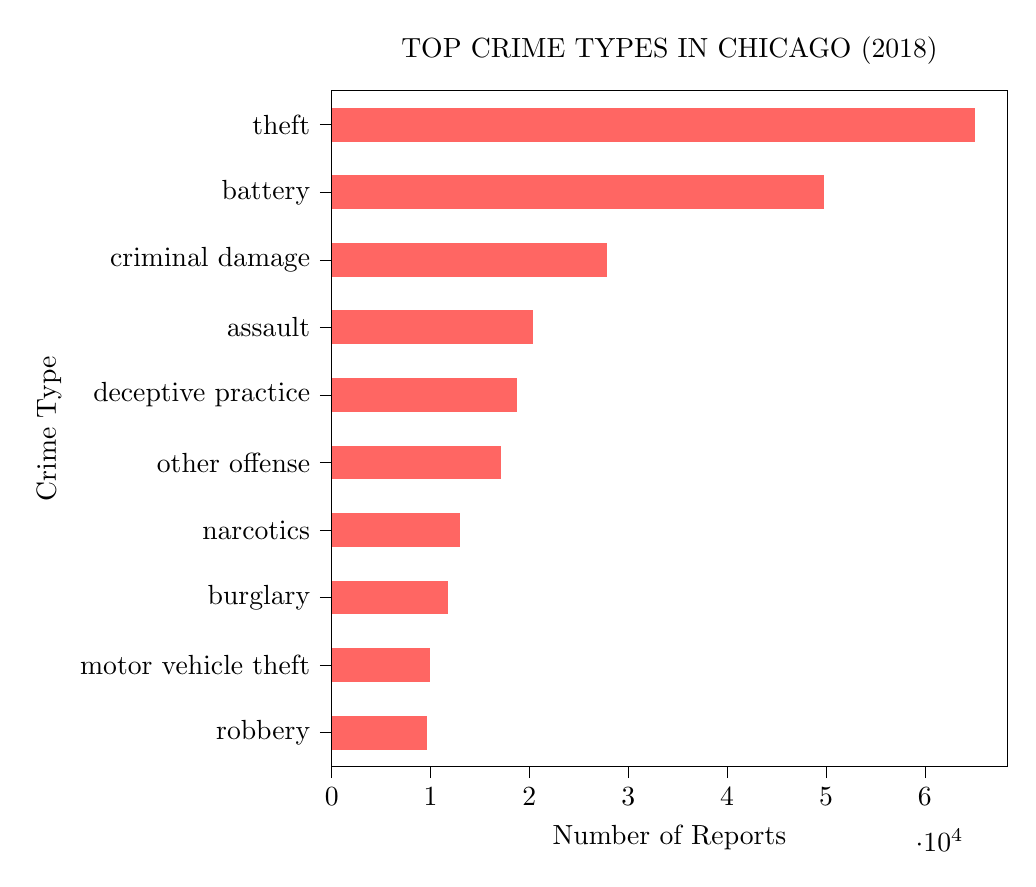
\begin{tikzpicture}

\definecolor{color0}{rgb}{1,0.4,0.388235294117647}

\begin{axis}[
height=4in,
tick align=outside,
tick pos=left,
title={\printsection{\MakeUppercase{Top Crime Types in Chicago (2018)}}},
width=4in,
x grid style={white!69.01960784313725!black},
xlabel={Number of Reports},
xmin=0, xmax=68332.95,
xtick style={color=black},
y grid style={white!69.01960784313725!black},
ylabel={Crime Type},
ymin=-0.5, ymax=9.5,
ytick style={color=black},
ytick={0,1,2,3,4,5,6,7,8,9},
yticklabels={robbery,motor vehicle theft,burglary,narcotics,other offense,deceptive practice,assault,criminal damage,battery,theft}
]
\draw[fill=color0,draw opacity=0] (axis cs:0,-0.25) rectangle (axis cs:9683,0.25);
\draw[fill=color0,draw opacity=0] (axis cs:0,0.75) rectangle (axis cs:9987,1.25);
\draw[fill=color0,draw opacity=0] (axis cs:0,1.75) rectangle (axis cs:11729,2.25);
\draw[fill=color0,draw opacity=0] (axis cs:0,2.75) rectangle (axis cs:12987,3.25);
\draw[fill=color0,draw opacity=0] (axis cs:0,3.75) rectangle (axis cs:17125,4.25);
\draw[fill=color0,draw opacity=0] (axis cs:0,4.75) rectangle (axis cs:18716,5.25);
\draw[fill=color0,draw opacity=0] (axis cs:0,5.75) rectangle (axis cs:20377,6.25);
\draw[fill=color0,draw opacity=0] (axis cs:0,6.75) rectangle (axis cs:27806,7.25);
\draw[fill=color0,draw opacity=0] (axis cs:0,7.75) rectangle (axis cs:49781,8.25);
\draw[fill=color0,draw opacity=0] (axis cs:0,8.75) rectangle (axis cs:65079,9.25);
\end{axis}

\end{tikzpicture}